\section{Analysis of the Synthetic Axion Data}\label{sec:faxion}
After TASEH finished collecting the CD102 data on November 15, 2021, 
the synthetic axion signals were injected into the cavity and read out via the 
same transmission line and amplification chain. The procedure 
to generate axion-like signals is summarized in 
Ref.~\cite{TASEHInstrumentation}. 
%Due to the uncertainties on the losses of signal transmission
% lines, the synthetic axion signals are not used to perform an absolute 
%calibration of the search sensitivity. Instead, 
A test with synthetic axion signals could be used to verify the procedures of 
data acquisition and physics analysis. The synthetic axion signals 
have a wider width (8~kHz) and longer tails compared to the line shape 
described by Eq.~\eqref{eq:simplesignal}. 
The expected SNR of the frequency bin with maximum power ($\approx 11\%$ of 
the total signal power), 
%synthetic axion signals, at 4.708970~GHz, was set to $\approx 3.35$.%, 
 at 4.70897~GHz, was set to $\approx 3.35$. 
%corresponding to a power of $\approx 6.03 \times 10^{-13}$~W in a 1-kHz 
%frequency bin.  
The total signal power injected 
corresponds to $\ggamma\approx 20 \left|g_\text{KSVZ}\right|$. 

The same analysis procedure as described in Sec.~\ref{sec:ana} is applied 
to the data with synthetic axion signals. 
Figure~\ref{fig:faxionstep} presents the individual raw power spectra in 
the 24 frequency scans. Before combining 
the 24 spectra, the SNR of the maximum-power bin from the scan with a resonant 
frequency closest to the injected signal is measured to be 
3.58. %the SNR is slightly higher than 3.35 due to a 
%5\% difference in the noise fluctuation between the measurements from 
%the calibration and the measurements taken right before injecting 
%axion-like signals. 
After the combination of the spectra and the merging of five frequency 
bins, the SNRs of the maximum-power bin increase to 4.74 and 6.12, 
respectively. Figure~\ref{fig:faxioncombinemerge} presents 
the SNR after the combination and the merging, respectively.    
%the 24 scans of the 
%synthetic axion data and the two 
%scans of the CD102 data are included and processed together. 
%
In order to 
validate the results of the SNRs, the analysis procedure is also applied  
to the simulated spectra that include both noise and a signal with the 
same power and the same line shape as those of the injected synthetic axions. 
The SNRs obtained with 200 simulations, before 
the combining, after the combining, and after the merging are %4.51 +/- 0.56% 
%3.56 +/- 0.47, 6.88 +/- 0.78
$3.6\pm 0.5$, $4.5\pm0.6$, and $6.9\pm0.8$, respectively, 
which are 
consistent with the results from the synthetic axion data.  
%In addition to the 
%injected synthetic axion signal, a candidate at 4.70801~GHz is found after 
%merging the spectra. Due to the limited access to the DR, 
%it is not possible to perform a rescan after the collection of the 
%synthetic axion data. Therefore,  
%the CD102 data from the two scans that had resonant frequencies close to 
%the candidate frequency are added so to mimic the rescan; the candidate is 
%found to be a statistical fluctuation.  
%Figures~\ref{fig:faxioncombine}--~\ref{fig:faxionmerge} present 
%the RDP spectra with the corresponding SNR, respectively, after combining 
%The analysis results of the synthetic axion signals prove that a power 
%excess of more than 5$\sigma$ can be found at the expected frequencies via 
%the standard analysis procedure. 
The consistency of the SNRs demonstrates 
the capability of the experimental setup and the analysis strategy to discover 
an axion signal with 
$\ggamma\approx {\cal O}\left(10\left|g_\text{KSVZ}\right|\right)$.


\begin{figure}[htbp]                                                                                                  
    \centering                                                                                                                       
    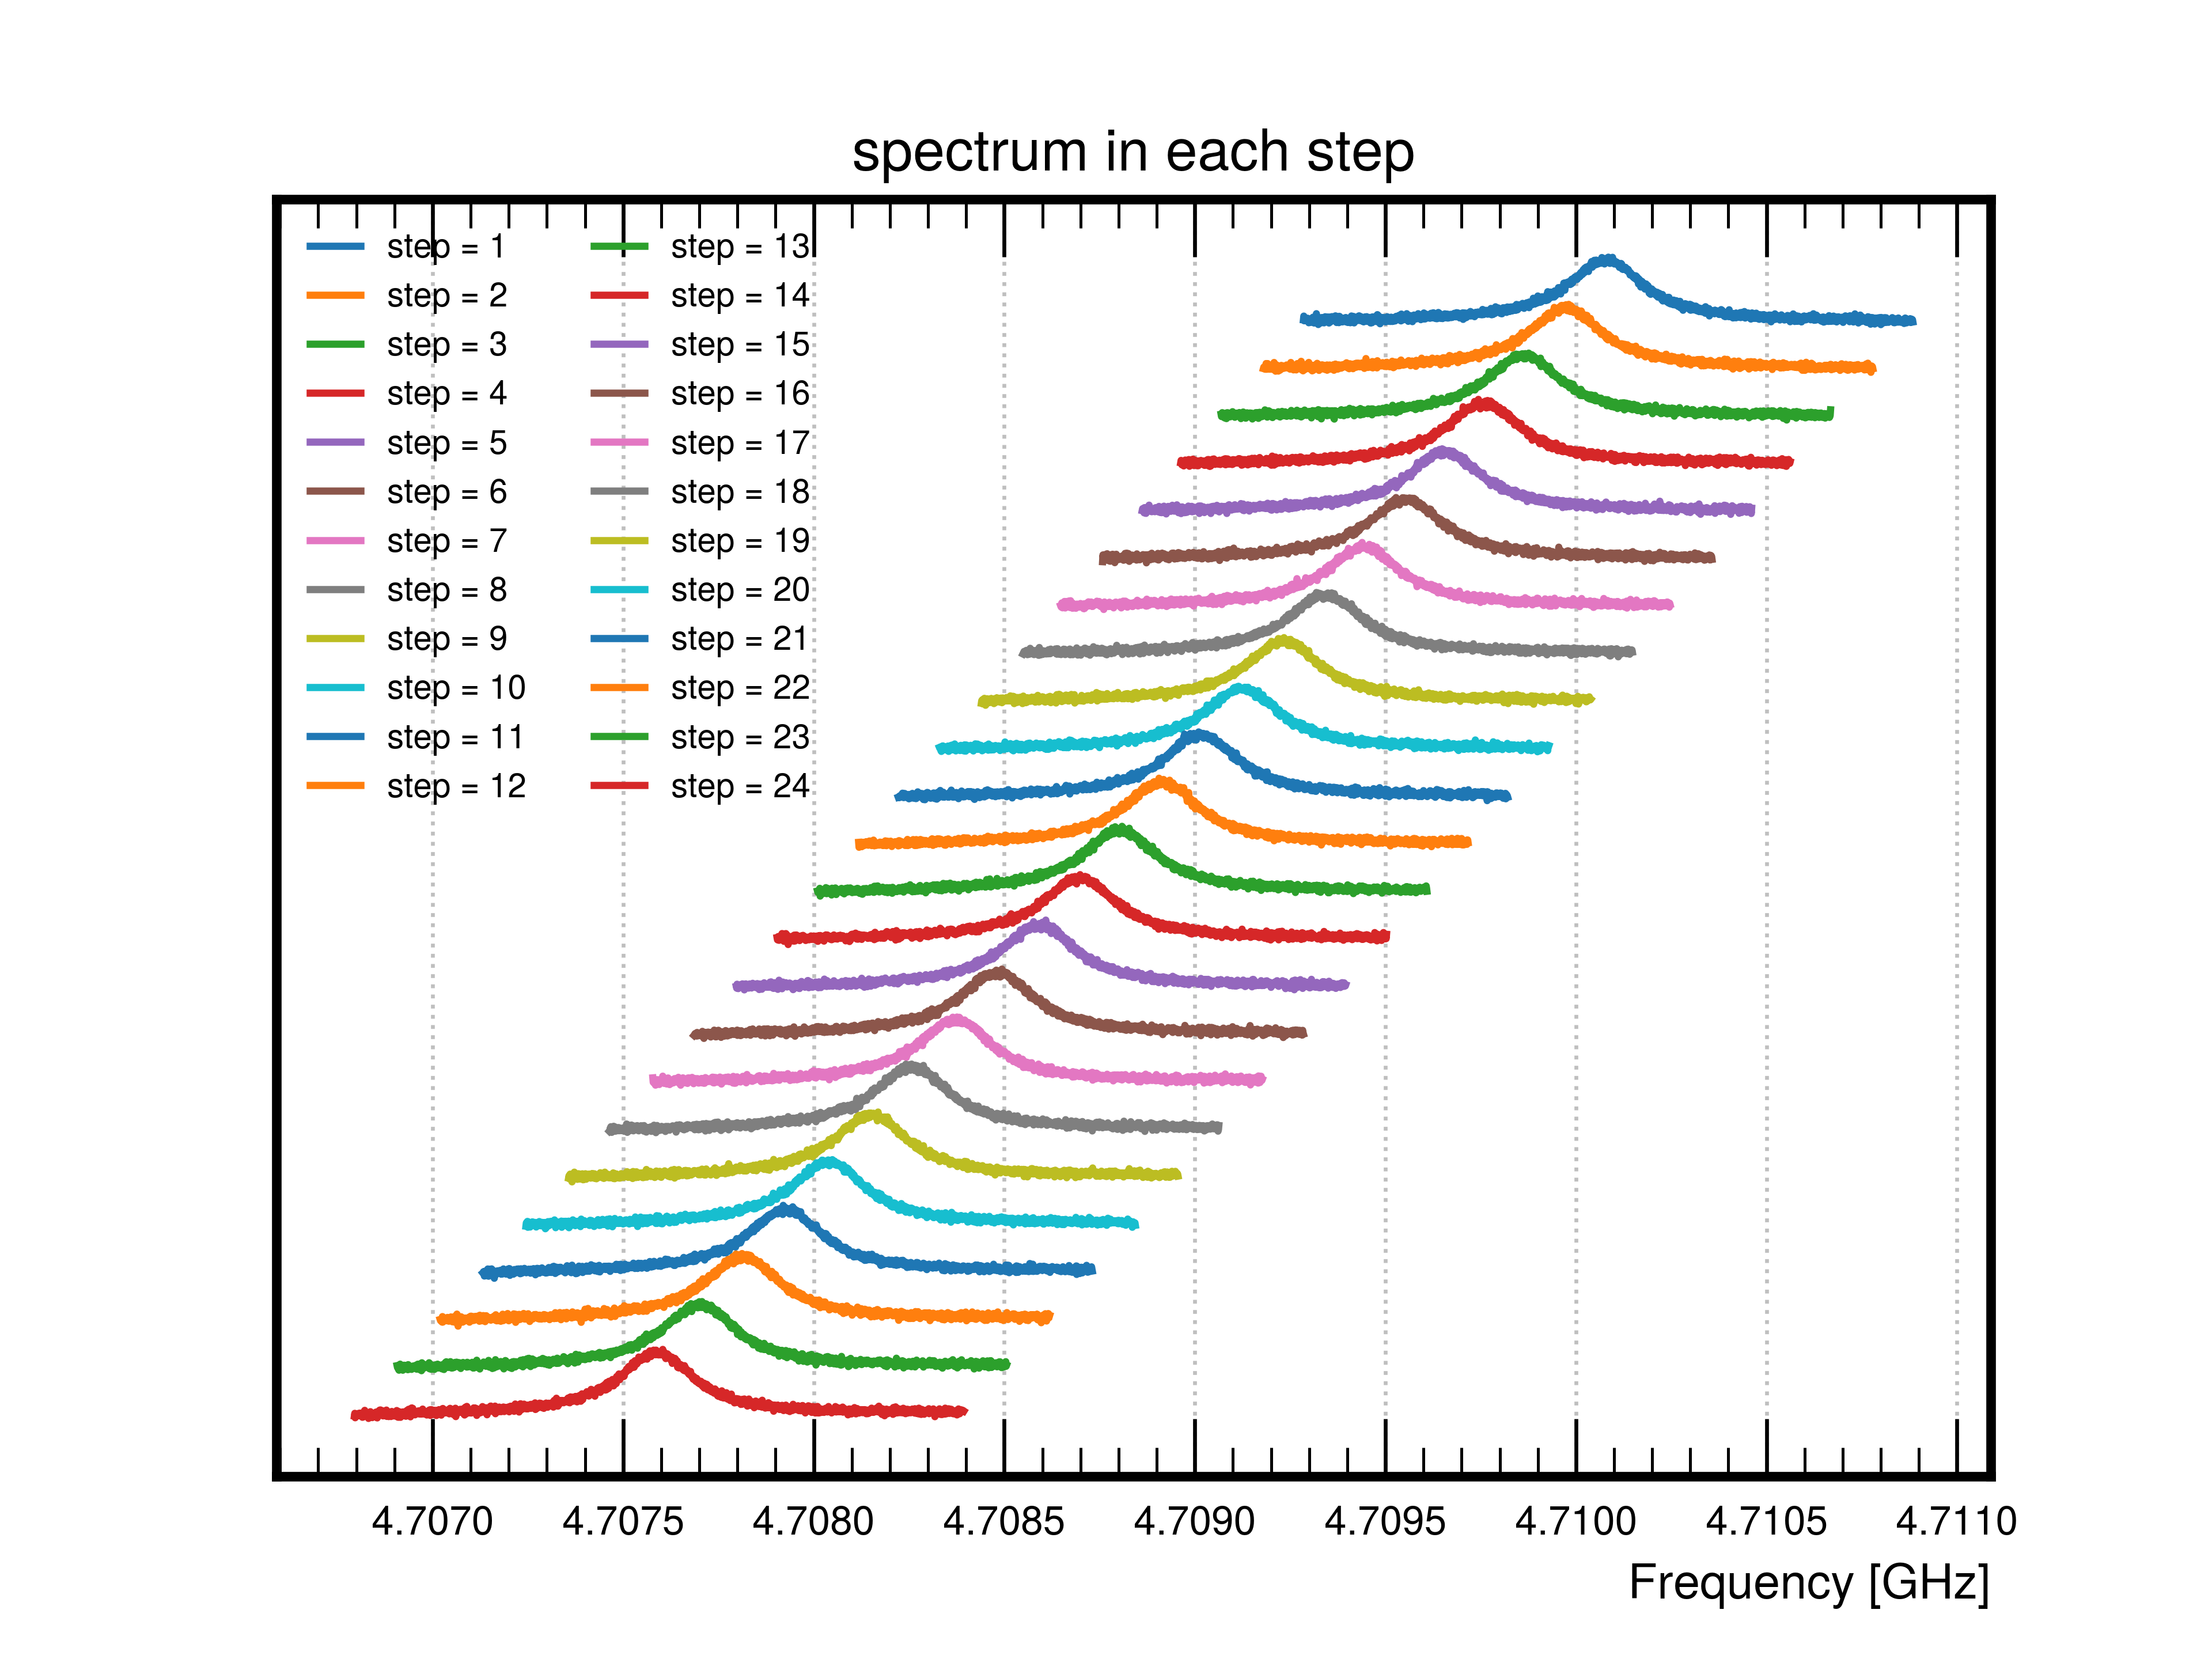
\includegraphics[width=8.6cm]{figures/faxion_rawpower_24steps.png}
 \caption{The raw output power spectra, before applying the 
 SG filter, from the 24 frequency steps of the synthetic axion 
data. In order to show the spectra clearly, the spectra are shifted 
with respect to each other with an arbitrary offset in the vertical scale.}                
\label{fig:faxionstep}                                                                                                            
\end{figure}                       

%\begin{figure}[htbp]                                                                                                  
%    \centering                                                                                                                       
%    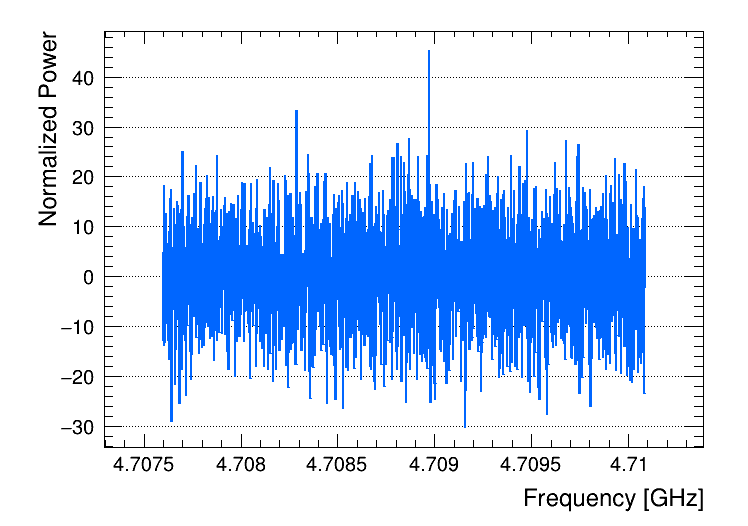
\includegraphics[width=8.6cm]{figures/Power_CombSpectrum_FaxionRun_AllSteps_Rescan_SG4_W201.png}
%    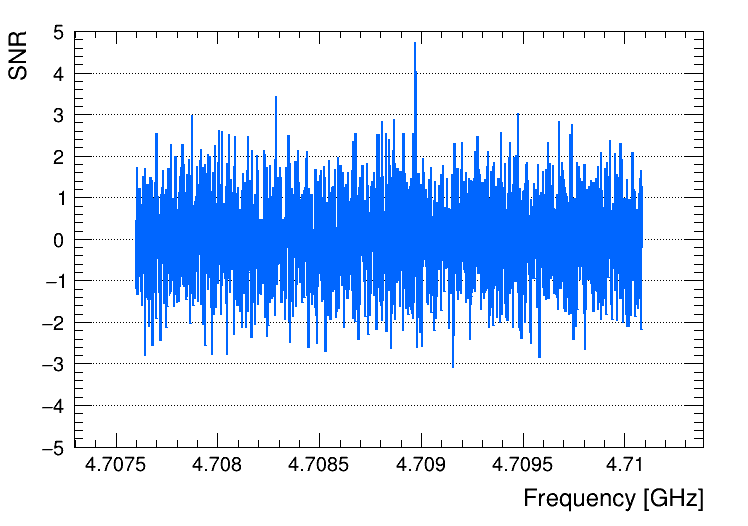
\includegraphics[width=8.6cm]{figures/SNR_CombSpectrum_FaxionRun_AllSteps_Rescan_SG4_W201.png}
%    \caption{The RDP (upper) and the 
%signal-to-noise ratio (lower) after combining the spectra 
%of the synthetic axion data with overlapping frequencies from different scans.
% The procedure and the weights for combination are summarized in 
%Sec.~\ref{sec:weighting_algorithm}.}                
%\label{fig:faxioncombine} 
%\end{figure}                       


%\begin{figure}[htbp]                                                   
%\centering                                                                                                                       
%   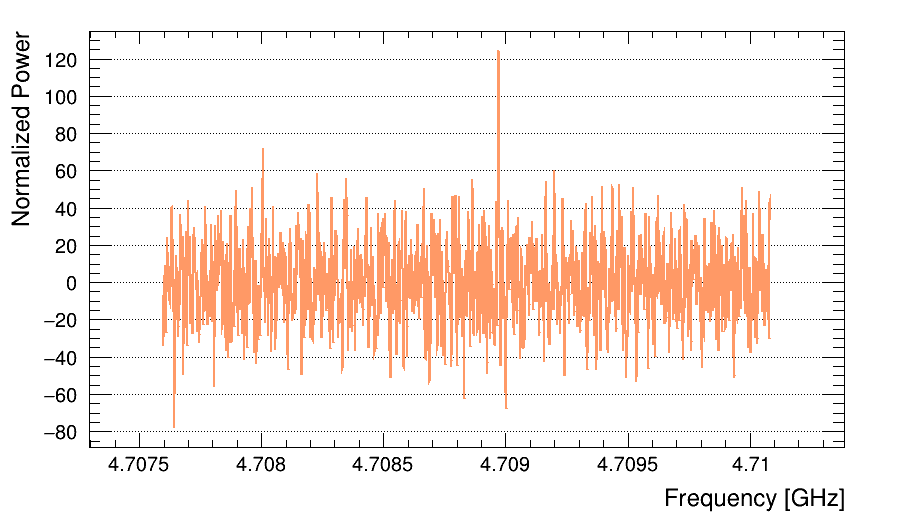
\includegraphics[width=8.6cm]{figures/Power_GrandSpectrum_FaxionRun_AllSteps_Rescan_Merged_5bin_SG4_W201_LqWeight.png}
%    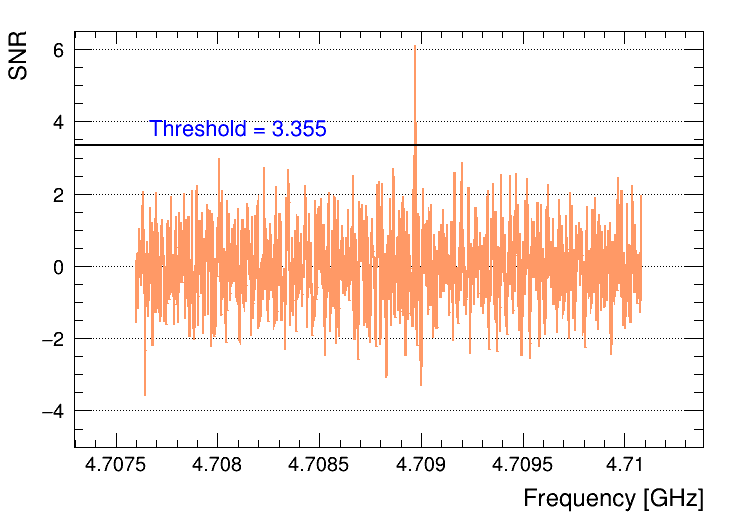
\includegraphics[width=8.6cm]{figures/SNR_GrandSpectrum_FaxionRun_AllSteps_Rescan_Merged_5bin_SG4_W201_LqWeight.png}
%    \caption{The RDP (upper) and the signal-to-noise ratio (lower) after 
%merging the RDP measured in five neighboring frequency bins of the 
%synthetic axion data. 
%The procedure and the weights for merging 
%are summarized in Sec.~\ref{sec:merge}.}                
%\label{fig:faxionmerge}    
%\end{figure}                       



\begin{figure}[htbp]                                                                                                  
    \centering                                                                                                                       
    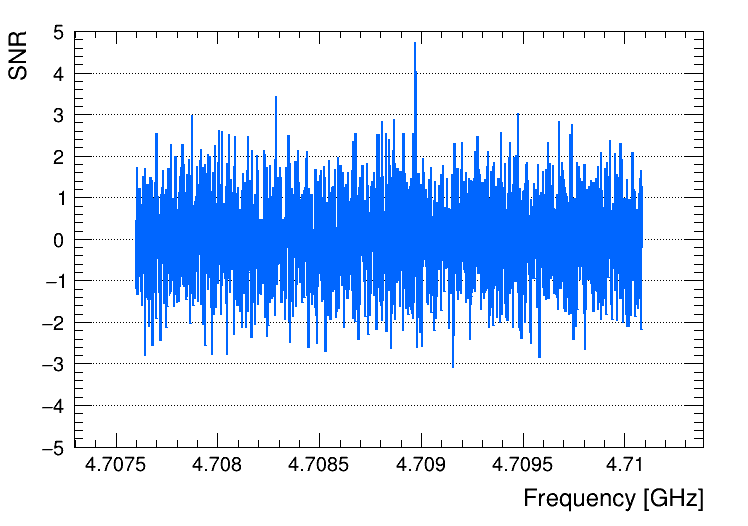
\includegraphics[width=8.6cm]{figures/SNR_CombSpectrum_FaxionRun_AllSteps_Rescan_SG4_W201.png}
    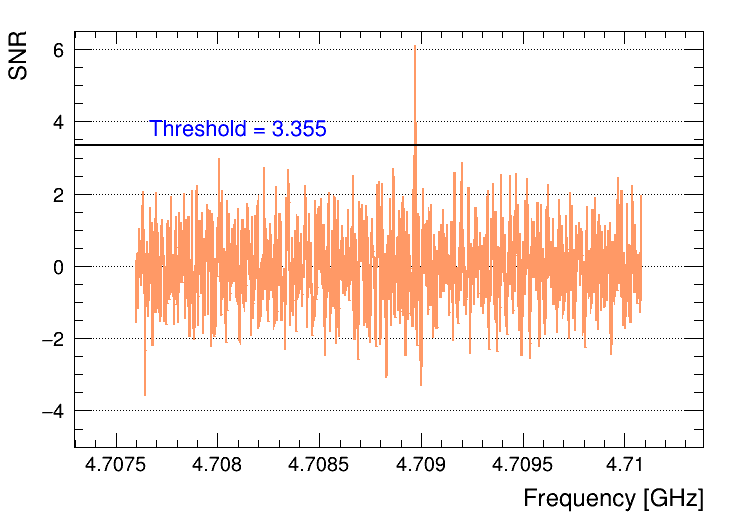
\includegraphics[width=8.6cm]{figures/SNR_GrandSpectrum_FaxionRun_AllSteps_Rescan_Merged_5bin_SG4_W201_LqWeight.png}
    \caption{The signal-to-noise ratio, from the synthetic axion data, 
after combining the spectra with overlapping frequencies from different 
scans (upper) and after merging the RDP measured in five neighboring 
frequency bins (lower). 
The procedure and the weights for combination and merging are summarized in 
Sec.~\ref{sec:weighting_algorithm} and Sec.~\ref{sec:merge}, respectively.}               
\label{fig:faxioncombinemerge} 
\end{figure}                       

   
